% !TEX encoding = UTF-8
% !TEX TS-program = pdflatex
% !TEX root = ../Tesi.tex
% !TEX spellcheck = it-IT

%************************************************
\chapter{Reciprocal Velocity Obstacle}
\label{cap:rvo}
%************************************************

Reciprocal Velocity Obstacle affronta il problema dell'oscillazione causato dal Velocity Obstacle incorporando la natura reattiva degli altri robot.

\section{Reciprocal Velocity Obstacle}
Per affrontare il problema delle traiettorie oscillatorie, invece di dover prendere tutte le responsabilit\'a, RVO lascia prendere al robot solo la met\'a della responsabilit\'a, per evitare le collisioni, pur assumendo che l'altro robot coinvolto ricambi prendendosi cura dell'altra met\'a.
\\L'idea base sarebbe di scegliere una nuova velocit\'a per ogni agente all'esterno degli altri Velocity Obstacle e che, questa nuova velocit\'a,  sia la media (\textit{average}) della velocit\'a corrente e di una velocit\'a che sia al di fuori degli Velocity Obstacle degli altri agenti. 

\subsection{Definition}

Questo principio \'e formalizzato come segue:

\begin{gather}
RVO_{A,B}({\boldsymbol{v}_ B}, {\boldsymbol{v}_A} ) =  \{ \boldsymbol{v'}_{A} | 2\boldsymbol{v'}_{A} - \boldsymbol{v}_{A} \in VO_{A,B}(\boldsymbol{v}_{B})  \}
\end{gather}

dove RVO\ped {A,B}({\bfseries\textit{v}\ped B},{\bfseries\textit{v}\ped A}) dell'agente \textit{B} su l'agente \textit{A} contiene tutte le velocit\'a per \textit{A} che saranno la media della velocit\'a corrente {\bfseries\textit{v}\ped A} e una velocit\'a all'interno di VO\ped{A,B}({\bfseries\textit{v}\ped B}) dell'agente \textit{B}. Pu\'o essere interpretato geometricamente come Velocity Obstacle, VO\ped{A,B}({\bfseries\textit{v}\ped B}),  traslato di $\tfrac{\boldsymbol{v}_ A + \boldsymbol{v}_ B}{2}$ dall'apice.

\section{Guarantees}
Proviamo che RVO possa essere usato per generare \textit{collision-free} e \textit{oscillation-free} per ogni agente.

\subsection{Collision-free Navigation}
Abbiamo {\bfseries\textit{v}\ped A} e {\bfseries\textit{v}\ped B} velocit\'a correnti, rispettivamente, di \textit{A} e \textit{B}, e permettiamo di scegliere ad entrambi la nuova velocit\'a ({\bfseries\textit{v'}\ped A} e {\bfseries\textit{v'}\ped B}) fuori da ogni 
Reciprocal Velocity Obstacle. Rispettando il \textit{teorema} e la \textit{legge} seguenti, essi ci garantiscono uno stato di \textit{safe} se e solo se entrambi gli agenti scelgono lo stesso lato (\textit{same side}) per passare ogni altro agente. 

\begin{teorema}[Collision-Free]

$\\{\boldsymbol{v'}_ A} \overrightarrow{\notin} RVO_{A,B}({\boldsymbol{v}_ B}, {\boldsymbol{v}_A} ) \wedge {\boldsymbol{v'}_ B} \overrightarrow{\notin} RVO_{B,A}({\boldsymbol{v}_ A}, {\boldsymbol{v}_B} ) \Rightarrow {\boldsymbol{v'}_ A} \overrightarrow{\notin} VO_{A,B}({\boldsymbol{v'}_ B}) \wedge {\boldsymbol{v'}_ B} \overrightarrow{\notin} VO_{B,A}({\boldsymbol{v'}_ A}) $
\end{teorema}

\begin{figure}
\centering 
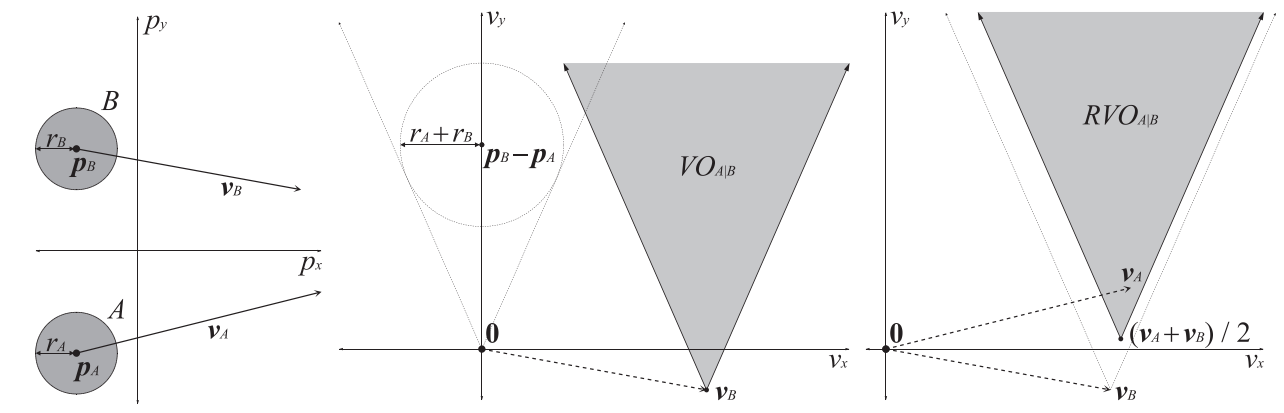
\includegraphics[width=0.8\columnwidth]{rvo} 
\caption[Costruzione del RVO rispetto al VO]{Costruzione del RVO rispetto al VO}
\label{fig:rvo} 
\end{figure}


\subsection{Same Side}
Possiamo garantire che entrambi gli agenti prenderanno automaticamente la nuova velocit\'a nello stesso lato, se ogni agente prender\'a la velocit\'a al di fuori di ogni RVO, tale che differisca del minimo possibile (\textit{closet}) dalla velocit\'a corrente dell'agente.
\\Ogni agente \textit{A} avr\'a una velocit\'a {\bfseries\textit{v}\ped A} + {\bfseries\textit{u}} \textit{closet} a {\bfseries\textit{v}\ped A} fuori dal RVO di \textit{B}, tale che B avr\'a {\bfseries\textit{v}\ped B} - {\bfseries\textit{u}} \textit{closet} a {\bfseries\textit{v}\ped B } fuori dal RVO di \textit{A}.
Se per \textit{A} questa \textit{closet} velocit\'a sar\'a sulla destra (o sinistra) di RVO di \textit{B}, allora \textit{B} sceglier\'a la \textit{closet} velocit\'a sullo stesso lato (e viceversa).\\Questo \'e provato dalla legge seguente:

\begin{legge}[Same Side]
\label{lex:sasi}
$\\ {\boldsymbol{v}_ A} + {\boldsymbol{u}} \notin RVO_{A,B}({\boldsymbol{v}_ B},{\boldsymbol{v}_ A}) \Leftrightarrow {\boldsymbol{v}_ B} - {\boldsymbol{u}} \notin RVO_{B,A}({\boldsymbol{v}_ A},{\boldsymbol{v}_ B})$
\end{legge}

\subsection{Oscillation-Free}

La scelta delle \textit{closet} velocit\'a, al di fuori degli RVO, garantisce la \textit{oscillation-free navigation} .Questo \'e provato dal teorema seguente:

\begin{teorema}[Oscillation-Free]

$\\{\boldsymbol{v}_ A} \in RVO_{A,B}({\boldsymbol{v}_ B}, {\boldsymbol{v}_A} ) \Leftrightarrow  {\boldsymbol{v}_ A} \in RVO_{A,B}({\boldsymbol{v}_ B - u }, {\boldsymbol{v}_A} + u )$
\end{teorema}

Quindi, la vecchia velocit\'a {\bfseries\textit{v}\ped A} di \textit{A} \'e all'interno del nuovo RVO di \textit{B}, dando le nuove velocit\'a {\bfseries\textit{v}\ped A} + {\bfseries\textit{u}} e {\bfseries\textit{v}\ped B} - {\bfseries\textit{u}} per l'agente \textit{A} e \textit{B}. Stesse premesse vengono rispettate per \textit{B}. 
Pertanto, dopo aver scelto la nuova velocit\'a, le vecchie candidate non saranno pi\'u valide e non verranno pi\'u scelte. Infatti, scegliendo la \textit{closet} velocit\'a fuori dal RVO di \textit{A} e di \textit{B}, gli RVO rimarranno esattamente nella stessa posizione.
Quindi {\bfseries\textit{v}\ped A} + {\bfseries\textit{u}} e {\bfseries\textit{v}\ped B} - {\bfseries\textit{u}} saranno ancora le velocit\'a pi\'u vicine alle velocit\'a preferite tra tutte quelle ammissibili. Di conseguenza non si verificheranno traiettorie oscillatorie.



